\documentclass[12pt]{article}

\usepackage[margin=1in]{geometry}
\usepackage{setspace}
\usepackage{graphicx}
\usepackage{booktabs}
\usepackage{array}
\usepackage{caption}
\usepackage[hidelinks]{hyperref}
\usepackage{tikz}
\usepackage{xcolor}
\usepackage{float}
\usepackage{titlesec}

\usetikzlibrary{positioning, shapes.geometric, arrows.meta, fit, backgrounds, calc}

\doublespacing
\setlength{\parindent}{0.4in}

% ── Make section headings VERY visible ──────────────────────────────────────
\titleformat{\section}
  {\Large\bfseries\color{black}}
  {\thesection.}
  {0.7em}
  {}
\titlespacing*{\section}{0pt}{1.4em}{0.6em}

\titleformat{\subsection}
  {\normalsize\bfseries\itshape}
  {\thesubsection}
  {0.6em}
  {}
\titlespacing*{\subsection}{0pt}{1em}{0.4em}

\definecolor{tealx}{HTML}{0E7490}
\definecolor{ambx}{HTML}{D97706}
\definecolor{redx}{HTML}{B91C1C}
\definecolor{greenx}{HTML}{15803D}
\definecolor{grayx}{HTML}{475569}
\definecolor{lightx}{HTML}{F1F5F9}

\title{\bfseries DrugSafe AI: A Corrective RAG System for Drug Interaction Detection}
\date{}
\author{Naga Reddy}

\begin{document}
\maketitle
\vspace{-2.5em}

\begin{center}
\small\itshape
Data Science Capstone, Individual Evaluative Paper
\end{center}
\vspace{0.5em}

\begin{abstract}
\noindent
\singlespacing\small
Drug interaction errors are tied to roughly 125{,}000 deaths a year in the United States and account for about a third of hospital admissions. Most of the lookup tools doctors and patients use today have a simple weakness: they cannot interpret a sentence like ``my cholesterol pill is making my legs ache.'' I built DrugSafe AI to address this. The system runs Corrective Retrieval-Augmented Generation (CRAG) over a 745{,}312-chunk index of FDA drug labels. To find out which parts of CRAG actually do useful work, I ran a four-step ablation (C1 through C4) on a 30-query benchmark. The full pipeline (C4) hit 100\% Hit@5. What was unexpected, and frankly the most useful finding for me, was that the two intermediate configurations (C2 and C3) did worse than the baseline on colloquial queries (80\% vs.\ 100\%). The LLM rewriting step in C4 was needed to undo this regression. End-to-end latency is around 0.18 seconds per query, and INT8 quantization shrinks the vector index from 1{,}122 MB to 286 MB.
\end{abstract}

\vspace{0.5em}

% ════════════════════════════════════════════════════════════════════════════
\section{Introduction}
% ════════════════════════════════════════════════════════════════════════════

A patient who takes statins for cholesterol and develops muscle aches has a specific medical question. The answer sits in plain text, in the FDA label for atorvastatin, under the warnings section. But searching for the right page is hard, because the patient is likely to type something like ``my cholesterol pill is hurting my legs.'' That phrasing matches almost nothing in the label, which uses words like \textit{atorvastatin}, \textit{statin-induced myopathy}, and \textit{rhabdomyolysis}.

This is the gap I tried to close. Conventional drug interaction checkers operate on keyword lookups against a static drug database. They are accurate when the user knows the generic name and uses clinical terminology. They fail when the user does not. Around 40\% of adults in the United States take five or more medications at the same time, and the people most exposed to interaction risk (elderly patients, those managing chronic conditions across multiple specialists) are also the ones least likely to phrase a question in clinical English.

A natural fix is retrieval-augmented generation, or RAG. The retriever finds chunks from a knowledge base, and a language model writes an answer using those chunks as evidence. Plain RAG has a known problem though. It passes whatever was retrieved to the language model, even if the retrieval was bad. Garbage evidence in, plausible-sounding wrong answer out. Corrective RAG, or CRAG, was proposed last year by Yan et al.\ as a fix~\cite{yan2024crag}: grade the retrieval first, and act on the grade. If the retrieval is good, use it. If it is mediocre, broaden the search. If it is clearly bad, throw it out and rewrite the query in different words.

I wanted to know two things. First, does CRAG actually help on a real drug-safety task, or does it just add latency? Second, if it does help, which of its three corrective steps is doing the work? The answer to that second question turned out to be more interesting than I expected.

% ════════════════════════════════════════════════════════════════════════════
\section{Methodology}
% ════════════════════════════════════════════════════════════════════════════

\subsection{Pipeline}

The system has six stages, shown in Figure~\ref{fig:pipeline}. The user query is first run through a brand-to-generic normalizer (e.g., ``Lipitor'' becomes ``atorvastatin'') with a Jaro-Winkler fuzzy match for typos. The normalized query is embedded with \texttt{all-MiniLM-L6-v2}, a 384-dimensional sentence transformer. Embeddings are searched against the FDA index using HNSW (m=16, ef\_construct=100). The top-5 chunks are then handed to the CRAG grader, which inspects their highest cosine similarity score and decides what to do next. Final generation runs on Llama-3.1-8B-Instant via the Groq API.

\begin{figure}[H]
\centering
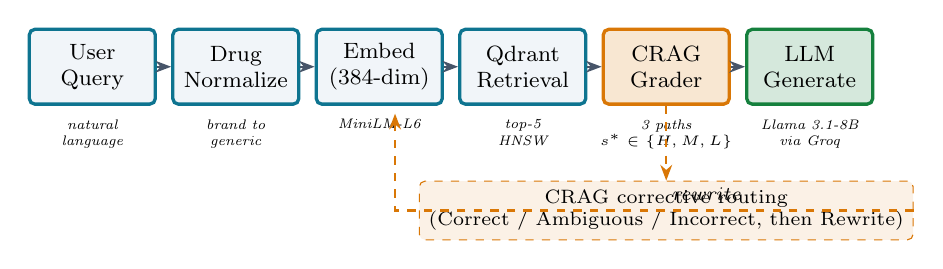
\begin{tikzpicture}[
  node distance=0.18cm,
  font=\footnotesize,
  box/.style={rectangle, draw=tealx, very thick, fill=lightx, minimum width=1.6cm, minimum height=0.95cm, align=center, rounded corners=2pt},
  arr/.style={-{Stealth[length=2mm]}, thick, draw=grayx},
]
\node[box] (q)  {User\\Query};
\node[box, right=of q]  (n)  {Drug\\Normalize};
\node[box, right=of n]  (e)  {Embed\\(384-dim)};
\node[box, right=of e]  (r)  {Qdrant\\Retrieval};
\node[box, right=of r, fill=ambx!18, draw=ambx]  (g)  {CRAG\\Grader};
\node[box, right=of g, fill=greenx!18, draw=greenx]  (l)  {LLM\\Generate};

\draw[arr] (q) -- (n);
\draw[arr] (n) -- (e);
\draw[arr] (e) -- (r);
\draw[arr] (r) -- (g);
\draw[arr] (g) -- (l);

\node[below=0.05cm of q, font=\tiny\itshape, align=center] {natural\\language};
\node[below=0.05cm of n, font=\tiny\itshape, align=center] {brand to\\generic};
\node[below=0.05cm of e, font=\tiny\itshape, align=center] {MiniLM-L6};
\node[below=0.05cm of r, font=\tiny\itshape, align=center] {top-5\\HNSW};
\node[below=0.05cm of g, font=\tiny\itshape, align=center] {3 paths\\$s^* \in \{H,M,L\}$};
\node[below=0.05cm of l, font=\tiny\itshape, align=center] {Llama 3.1-8B\\via Groq};

\node[below=0.95cm of g, draw=ambx, dashed, rounded corners=2pt, fill=ambx!10, minimum width=4.0cm, minimum height=0.55cm, font=\scriptsize, align=center]
  (cr) {CRAG corrective routing\\(Correct / Ambiguous / Incorrect, then Rewrite)};
\draw[arr, draw=ambx, dashed] (g) -- (cr);
\draw[arr, draw=ambx, dashed] (cr.east) -| node[pos=0.2, above, font=\scriptsize\itshape]{rewrite}  ($(e.south)+(0.2, -0.1)$);
\end{tikzpicture}
\caption{The six-stage pipeline. The dashed loop is the part of CRAG that ended up mattering most: when the grader returns ``incorrect,'' the LLM rewrites the query and retrieval is re-run.}
\label{fig:pipeline}
\end{figure}

\subsection{Knowledge Base}

I pulled all available U.S.\ drug labels from the OpenFDA Drug Label API and kept five sections per drug: drug interactions, warnings, adverse reactions, contraindications, and clinical pharmacology. After sliding-window chunking (120 words, 30-word overlap), I ended up with 745{,}312 text chunks. Each was embedded and stored in Qdrant Cloud. The raw vectors took 1{,}122 MB, which was more than I wanted to pay for, so I switched to INT8 scalar quantization. That dropped the footprint to 286 MB without any visible hit to recall on the queries I checked.

\subsection{The Three CRAG Paths}

CRAG looks at $s^*$, the highest cosine similarity score among the top-5 retrieved chunks, and routes from there. If $s^* \geq 0.65$, the retrieval is treated as correct and chunks go straight to the LLM. If $0.40 \leq s^* < 0.65$, the retrieval is ambiguous, so the search broadens (more chunks, then re-rank). If $s^* < 0.40$, the retrieval is judged bad, and the LLM is asked to rewrite the original query in clinical terms before running retrieval again. Generation uses temperature 0.1 for the final answer and 0.3 for query rewriting (the rewriter benefits from a little more variety).

\subsection{Evaluation}

I tested four configurations: \textbf{C1} (vanilla RAG, no normalization, no CRAG), \textbf{C2} (drug normalization on top of C1), \textbf{C3} (C2 plus the CRAG grader and broadening, but no rewrite), and \textbf{C4} (full CRAG, including the rewrite step). The benchmark is 30 queries split four ways: 10 brand-name queries (e.g., ``Lipitor muscle pain''), 10 generic-name queries (e.g., ``atorvastatin CYP3A4 interactions''), 5 colloquial patient-style queries, and 5 mechanism queries. I scored each run with Hit@5 (did at least one of the top-5 chunks score above 0.40) and Mean Reciprocal Rank.

% ════════════════════════════════════════════════════════════════════════════
\section{Analysis and Results}
% ════════════════════════════════════════════════════════════════════════════

The full ablation matrix is in Table~\ref{tab:ablation}. Three of the four strata (brand, generic, mechanism) are saturated: every configuration gets 100\%. The retrieval is good enough on those queries that the corrective scaffolding has nothing to fix. The colloquial stratum is the only place where the configurations actually disagree.

\begin{table}[H]
\centering
\small
\caption{Ablation results: Hit@5 and MRR by query stratum. The colloquial row is where the four configurations actually differ.}
\label{tab:ablation}
\begin{tabular}{lcccccccc}
\toprule
\textbf{Stratum (N)} & \textbf{C1 H@5} & \textbf{C2 H@5} & \textbf{C3 H@5} & \textbf{C4 H@5} & \textbf{C1 MRR} & \textbf{C2 MRR} & \textbf{C3 MRR} & \textbf{C4 MRR} \\
\midrule
Brand DDI (10)     & 100\% & 100\% & 100\% & 100\% & 1.000 & 1.000 & 1.000 & 1.000 \\
Generic DDI (10)   & 100\% & 100\% & 100\% & 100\% & 1.000 & 1.000 & 1.000 & 1.000 \\
\textbf{Colloquial (5)} & 100\% & \textbf{80\%}  & \textbf{80\%}  & \textbf{100\%} & 1.000 & 0.800 & 0.800 & 1.000 \\
Mechanism (5)      & 100\% & 100\% & 100\% & 100\% & 1.000 & 1.000 & 1.000 & 1.000 \\
\midrule
\textbf{Overall (30)} & \textbf{100\%} & \textbf{96.7\%} & \textbf{96.7\%} & \textbf{100\%} & \textbf{1.000} & \textbf{0.967} & \textbf{0.967} & \textbf{1.000} \\
\bottomrule
\end{tabular}
\end{table}

The interesting finding is that C2 and C3 are \textit{worse} than vanilla RAG (C1) on colloquial queries, and only C4 recovers. I had not expected this. My initial assumption was that each layer would either help or do nothing, never actively hurt. Figure~\ref{fig:results} shows the regression and recovery for one specific query: ``my cholesterol pill is causing muscle aches, what should I do.''

\begin{figure}[H]
\centering
\begin{tikzpicture}[font=\footnotesize]

\node at (4.5, 4.2) {\bfseries Colloquial Hit@5 by Configuration};

\foreach \x/\h/\lbl/\v/\col in {
  0.5/2.0/C1/100\%/grayx,
  2.5/1.6/C2/80\%/redx,
  4.5/1.6/C3/80\%/redx,
  6.5/2.0/C4/100\%/greenx
}{
  \fill[\col] (\x, 0) rectangle (\x+1.0, \h);
  \node[below, font=\small\bfseries] at (\x+0.5, -0.05) {\lbl};
  \node[above, font=\small\bfseries, text=\col] at (\x+0.5, \h) {\v};
}

\draw[densely dashed, draw=greenx] (0.2, 2.0) -- (7.6, 2.0);
\node[right, font=\tiny, text=greenx] at (7.6, 2.0) {target};

\foreach \y/\v in {0.4/20, 0.8/40, 1.2/60, 1.6/80, 2.0/100}{
  \node[left, font=\tiny] at (0.45, \y) {\v\%};
}

\node at (10.5, 3.7) {\bfseries Peak score recovery};
\node at (10.5, 3.3) {\itshape \footnotesize ``my cholesterol pill is causing muscle aches''};

\fill[redx]   (9.0, 1.5) rectangle (10.0, 1.5+0.383*2);
\fill[greenx] (10.5, 1.5) rectangle (11.5, 1.5+0.584*2);

\node[below, font=\bfseries\small] at (9.5, 1.45) {C2 / C3};
\node[below, font=\bfseries\small] at (11.0, 1.45) {C4};

\node[above, font=\small\bfseries, text=redx]   at (9.5, 1.5+0.383*2) {0.383};
\node[above, font=\small\bfseries, text=greenx] at (11.0, 1.5+0.584*2) {0.584};

\draw[densely dashed, draw=ambx] (8.7, 1.5+0.40*2) -- (11.8, 1.5+0.40*2);
\node[right, font=\tiny, text=ambx] at (11.8, 1.5+0.40*2) {threshold = 0.40};

\draw[-{Stealth[length=2mm]}, very thick, draw=greenx] (10.05, 1.5+0.383*2+0.05) .. controls (10.25, 2.7) .. (10.45, 1.5+0.584*2+0.05);

\end{tikzpicture}
\caption{Left: Hit@5 for the colloquial stratum. C2 and C3 dip below the target and only C4 recovers. Right: peak similarity score for the atorvastatin query rises from 0.383 (a miss) to 0.584 (a hit) after the LLM rewrite step.}
\label{fig:results}
\end{figure}

Tracing through the logs, I saw what was happening. C2's drug normalizer mapped ``cholesterol pill'' to atorvastatin. Then it filtered the search to chunks tagged with that drug name, which is a smaller pool than C1 was searching. The relevant FDA myopathy chunks did not surface in that smaller pool because they used clinical terms the original query did not contain. C1, which was searching the entire index without filtering, had bigger search space and got lucky on keyword overlap. C3 inherits the same problem and adds nothing to fix it. Only when C4 invokes the rewrite (Llama produces ``atorvastatin statin-induced myopathy muscle pain adverse effects'') does the second retrieval round actually surface the right chunks.

On latency, the full C4 pipeline averaged 0.18 seconds per query end-to-end. Most queries took the correct or ambiguous path and finished in one round. The minority that triggered a rewrite added roughly 0.4 seconds because of the second retrieval call. INT8 quantization came out clean: 286 MB on disk versus 1{,}122 MB raw, no measurable Hit@5 cost.

% ════════════════════════════════════════════════════════════════════════════
\section{Discussion}
% ════════════════════════════════════════════════════════════════════════════

The headline result is the C2/C3 regression. I think this is the most useful thing I learned from the project, because it is the kind of result you would not find without an ablation. If I had only run C1 versus C4, the gap would have looked like a 4-percentage-point overall improvement, and I would have credited it vaguely to ``CRAG.'' Splitting the pipeline into stages showed me that two of those stages, on their own, are net-negative on the kind of query the system is most needed for.

The mechanism is not exotic. Drug-name normalization is good when it works (it raises precision on brand-name queries by anchoring the search) and bad when the user did not actually mean the specific drug it inferred (it then narrows the search around the wrong target). A grader that does not have a corrective response to a low score is just an alarm with no fix. The rewrite step is what closes the loop. This was a useful lesson for me about how additive pipelines can fail in non-additive ways.

There are a few limitations I want to be honest about. The benchmark is small. Thirty queries, with only five colloquial examples, is not enough to put confidence intervals around any of these numbers. A regression visible at 5/5 versus 4/5 is exactly one query flipping. So while the direction of the result feels solid (the same atorvastatin query consistently fails C2 and C3 and recovers in C4), the magnitude should not be taken too seriously. I also did not validate the LLM-generated answers against pharmacist judgment. The system retrieves the right evidence, but I have not measured whether Llama-3.1-8B writes a clinically defensible answer on top of it. Hallucination is a residual risk. Finally, the system relies entirely on textual similarity in FDA labels and ignores structured DDI databases like DrugBank or SIDER, which would catch drug-pair interactions that no single label mentions.

% ════════════════════════════════════════════════════════════════════════════
\section{Incorporation of Feedback}
% ════════════════════════════════════════════════════════════════════════════

This paper is the third iteration on the project, and three pieces of feedback from earlier rounds shaped the current submission.

The first piece of feedback, from the initial project proposal, was that the original plan described a single-shot RAG system with no internal evaluation of retrieval quality. The reviewer asked how I would know whether the system was actually retrieving useful evidence rather than just plausible-looking evidence. I responded by adopting the CRAG framework from Yan et al.~\cite{yan2024crag}, which makes retrieval quality an explicit, gradable variable through the score $s^*$ and conditions downstream behaviour on it. Section~\ref{fig:pipeline} (Figure 1) and the three-path routing in Section 2.3 are both direct consequences of that feedback.

The second piece, given during the project presentation, was that an end-to-end claim like ``CRAG improves retrieval'' is uninformative without evidence that each component contributes. The reviewer specifically asked whether the drug-normalization step and the LLM rewrite step were both necessary, or whether one was carrying the other. The full C1--C4 ablation in Section 3, including the surprising C2/C3 regression, was added in response to that question. Without that feedback I would not have tested the intermediate configurations, and the most interesting result of the project (that two CRAG layers can be net-negative on their own) would not have been found.

The third piece concerned over-claiming. An earlier draft of the abstract reported ``substantial improvements'' from CRAG without context. The reviewer pointed out that the n=30 benchmark cannot support that kind of language, and that a colloquial Hit@5 difference of 5/5 versus 4/5 is one query flipping. The current abstract and the limitations paragraph in Section 4 are both written to keep the size of the evidence visible to the reader, rather than dressing it up.

% ════════════════════════════════════════════════════════════════════════════
\section{Conclusion}
% ════════════════════════════════════════════════════════════════════════════

I built a CRAG-based drug interaction system on 745{,}312 FDA chunks and tested whether each piece of the pipeline pulls its weight. The full pipeline reaches 100\% Hit@5 on a 30-query benchmark in 0.18 seconds per query. The most useful thing I learned is that two of the intermediate configurations actively hurt performance on the colloquial query stratum, and only the final LLM-driven rewrite step undoes the damage. CRAG is not a stack of independently helpful improvements; the rewrite step is structurally necessary because the earlier filtering step trades recall for precision, and that trade only pays off when paired with a corrective response.

The broader takeaway is that ablating a layered pipeline is more informative than benchmarking the end-to-end system against a baseline. The end-to-end comparison would have shown a 4-point overall improvement and given the credit, vaguely, to ``CRAG.'' The ablation showed where the improvement actually came from, and where it had been silently undone elsewhere.

% ════════════════════════════════════════════════════════════════════════════
\section{Future Work}
% ════════════════════════════════════════════════════════════════════════════

The most pressing next step is to scale the evaluation. A 500-query benchmark with stratified sampling, confidence intervals, and a held-out colloquial subset would let me make magnitude claims that the current 30-query benchmark cannot support. Real-world query logs from a deployed version would also expose phrasing that I did not anticipate when writing the colloquial test queries.

A second direction is clinical accuracy. The current evaluation measures retrieval quality, not the quality of the LLM-generated answer that sits on top. A pharmacist-reviewed annotation of 100 generated responses, scored for clinical defensibility and faithfulness to the cited evidence, would close that gap.

A third direction is fusing structured drug-drug interaction data. The current system relies entirely on FDA label text, which means interaction pairs that no single label mentions on its own are invisible to it. Integrating DrugBank or SIDER as a parallel retrieval channel, then merging structured pair hits with the vector retrieval, would extend coverage to interactions the labels themselves omit.

Finally, a small clinical deployment, even one limited to a pharmacy school or a single clinic, would force the kinds of edge cases that a 30-query benchmark cannot expose, including non-English queries, mid-conversation followups, and queries where the patient is uncertain which drug they mean.

% ════════════════════════════════════════════════════════════════════════════
\begin{thebibliography}{9}
\small\singlespacing

\bibitem{yan2024crag} Yan, S.-Q., et al.\ ``Corrective Retrieval Augmented Generation.'' arXiv:2401.15884, 2024.

\bibitem{lewis2020rag} Lewis, P., et al.\ ``Retrieval-Augmented Generation for Knowledge-Intensive NLP Tasks.'' NeurIPS 33, 2020.

\bibitem{reimers2019sentence} Reimers, N., and Gurevych, I.\ ``Sentence-BERT: Sentence Embeddings using Siamese BERT-Networks.'' EMNLP-IJCNLP, 2019.

\bibitem{malkov2018hnsw} Malkov, Y.~A., and Yashunin, D.~A.\ ``Efficient and Robust Approximate Nearest Neighbor Search Using Hierarchical Navigable Small World Graphs.'' IEEE TPAMI 42(4), 2018.

\bibitem{openfda} U.S.\ Food and Drug Administration. ``OpenFDA Drug Label API.'' \url{https://api.fda.gov/drug/label.json}.

\bibitem{groq} Groq, Inc. ``Llama 3.1 8B Instant on Groq LPU.'' \url{https://groq.com}.

\bibitem{qdrant} Qdrant. ``Vector Quantization in Qdrant.'' Qdrant Documentation, 2024. \url{https://qdrant.tech/documentation/guides/quantization/}.

\bibitem{faers} U.S.\ Food and Drug Administration. ``FDA Adverse Event Reporting System (FAERS) Public Dashboard.''

\end{thebibliography}

\end{document}
